In this problem, we are going to learn the class of $k$-decision
lists. A decision list is an ordered sequence of if-then-else
statements. The sequence of if-then-else conditions are tested in
order, and the answer associated to the first satisfied condition is
output. See Figure~\ref{fig:decision_list} for an example of a
$2$-decision list.

\begin{figure}[h]
\begin{center}
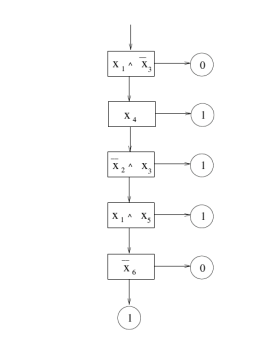
\includegraphics[width=1.35in]{auto/figure.png}
\caption{A $2$-decision list.}
\label{fig:decision_list}
\end{center}
\end{figure}

A {\em $k$-decision list} over the variables $x_{1}, \ldots, x_{n}$ is
an ordered sequence $L=(c_{1}, b_{1}), \ldots, (c_{l},b_{l})$ and a
bit $b$, in which each $c_{i}$ is a conjunction of at most $k$
literals over $x_{1},\ldots, x_{n}$. The bit $b$ is called the {\em
  default} value, and $b_{i}$ is referred to as the bit {\em
  associated} with condition $c_{i}$. For any input $x \in \{0,
1\}^{n}$, $L(x)$ is defined to be the bit $b_{j}$, where $j$ is the
smallest index satisfying $c_{j}(x)=1$; if no such index exists, then
$L(x)=b$.

We denote by $k\mbox{\em -DL}$ the class of concepts that can be
represented by a $k$-decision list.


\begin{enumerate}
\item \relax[8 points] Show that if a concept $c$ can be represented
  as a $k$-decision list so can its complement, $\neg c$. You can show
  this by providing a $k$-decision list that represents $\neg c$,
  given $c = \{(c_{1},b_{1}), \ldots, (c_{l},b_{l}),b)$.
\begin{solution}
A k-decision list is represented by $c = \{(c_{1},b_{1}), \ldots, (c_{l},b_{l}),b)$. The complement of $c$ can be written as $\neg c = \{(c_{1}, \neg b_{1}), \ldots, (c_{l},\neg b_{l}),\neg b)$. which is also a k-decision list. The default value of each $c_{i}$ conjunction is complemented.
\end{solution}
\item \relax[9 points] Use  Occam's Razor to show: \\
  For any constant $k \geq 1$, the class of $k$-decision lists is
  PAC-learnable.
\begin{solution}
To prove that class of k-decision list is PAC-learnable, we have to bound the size of the hypothesis space H.
In k-decision list each conjunction has atmost k-literals.
No of such conjunctions =
\[ |\mathcal{C}| = \sum_{i=1}^k {n\choose i}.2^i = \mathcal{O}(n^k) \]  
now either of the conjunction can have a bit value $b$ as $0$ or $1$ or it can be absent in the k-decision list. So we have three choices. The conjunctions can also be arranged in any order, which is a permutation.
Hence:
\[ |\mathcal{H}| = 3^{|\mathcal{C}|} |\mathcal{C}|!\] 
\[ \log(|\mathcal{H}|) = \log( (3^{|\mathcal{C}|} |\mathcal{C}|!)\]
since factorial will be dominant term among all:
\[ \log(|\mathcal{H}|) = \mathcal{O}(k.n^klog(n))  \]
using Occam's razor:
number of training samples 
\[ M > \frac{1}{\epsilon }( \ln \frac{1}{\delta} + \log(|\mathcal{H}|)) \]
using $|\mathcal{H}|$:
\[ M > \frac{1}{\epsilon }( \ln \frac{1}{\delta} + \mathcal{O}(k.n^klog(n)) \]
which is polynomial in $n$ number of literals. So the k-DL is PAC-learnable.
\end{solution}
\item \relax[8 points] Show that $1$-decision lists are a linearly
  separable functions. (Hint: Find a weight vector that will make the
  same predictions a given $1$-decision list.)
\begin{solution}
Let there be $l$ literals that appear in the 1-DL from top to bottom denoted by  $x_1,x_2,...,x_l$.  Let $b_1,b_2,...,b_l$  denotes the polarities associated with them in the 1-DL. we can set $b_i = -1$ if $x_i$ is appears with zero bit  or $b_i = 1$ otherwise.
Now we can create a linear threshold function: 
\[ sign( w^T  x + \theta ) \ge 0  \] 
that makes the same decisions as the decision list. Let $\bw \in \mathcal{R}^l$ be the weight vector.The ith component of the weight vector is $w_i = b_i 2^{l+1-i}$.If the default value of the 1-DL is false then set threshold $\theta$ to $-1$. Otherwise $\theta=1$. 

Note that we built the weight vector based on literals that appear in the decision list. Instead,if we construct the weight vector based on $x$, we should represent $x$ as a $2n$ dimension vector
$[x_1,\neg x_1, x_2,\neg x_2,....., x_n,\neg x_n]$, and set all weights in $w \in R^{2n}$ corresponding to the literals that do not appear in the 1-DL to zero.\\
The key point to notice about the design of this linear threshold function is that the weights must decrease geometrically as you go down the decision list so that the current feature's weight dominates all the weights that come after it whenever all the features that came before it were inactive. Note that the threshold has been set so that when all features are inactive, the prediction of the linear threshold function is the same as that of the 1-DL.
\end{solution}
\end{enumerate}



%%% Local Variables: 
%%% mode: latex
%%% TeX-master: "hw3"
%%% End: 
